\documentclass{article}
\usepackage{amsmath}
\usepackage{amssymb}
\usepackage{booktabs}
\usepackage{listings}
\usepackage{graphicx}
\usepackage{float}
\usepackage{array}
\usepackage{graphicx}
\usepackage{hyperref}



\title{Assignment: The Mystery Box Effect in Consumer Behavior }
\author{Margarita Gusakova (155403) \\
        Haroon Rashid (158448) }
\date{\today}

\begin{document}

\maketitle

\section{Introduction}
A \textbf{\emph{mystery box}} is a product offered at a fixed price with uncertain content, where consumers knowingly accept incomplete information about product characteristics at the moment of purchase.

\textit{Do you think the mystery box will be on average better / equal / worse than the known box?}

In standard economic theory, consumers are assumed to evaluate goods based on their expected utility, which depends on known attributes such as quality, quantity, and price. Under this framework, uncertainty about a product’s characteristics should not increase its valuation, and may even reduce it due to risk or ambiguity aversion. However, a growing body of evidence in behavioral economics suggests that real-world consumer behavior often deviates from these predictions, particularly when decisions involve uncertainty, emotions, and psychological biases.

One prominent example of such deviations is the increasing popularity of \emph{mystery boxes} or \emph{blind products}, where consumers purchase goods without knowing their exact contents in advance. Mystery boxes are widely used in marketing strategies across industries, including food, fashion, and digital goods, despite the fact that their expected monetary value is often comparable to, or even lower than, that of equivalent products with known characteristics. This raises an important behavioral question: \emph{why are consumers sometimes willing to pay more for products with uncertain outcomes?}

From a behavioral perspective, several mechanisms may explain this phenomenon. First, uncertainty may generate intrinsic utility through curiosity and anticipation, consistent with the information-gap theory, according to which individuals derive pleasure from resolving uncertainty. Second, mystery products may trigger affective responses such as excitement or surprise, leading consumers to rely on heuristics rather than deliberate evaluation. Third, consumers may overweight the probability of receiving a particularly desirable outcome, reflecting biased probability weighting under uncertainty.

The objective of this project is to study whether consumers exhibit a higher willingness to pay (WTP) for a mystery box of chocolate compared to a box with known contents, holding constant the general product category. Using data from a randomized online survey, we compare stated WTP across individuals exposed to a mystery condition and a known-product condition. By doing so, we aim to contribute to the behavioral literature on valuation under uncertainty and to provide empirical evidence on the role of mystery and ambiguity in consumer decision-making.

\section{Research Design and Instruments}
\subsection{Overall approach}
We study the \emph{mystery box effect} using a randomized online survey experiment. The research design follows a between-subjects structure: each respondent is exposed to only one scenario, which allows us to compare valuations across conditions without contamination from direct comparisons.

\subsection{Experimental treatments}
Participants are randomly assigned to one of two conditions:

\begin{itemize}
    \item \textbf{Known Box (Control):} respondents evaluate a chocolate box with clearly specified contents.
    \item \textbf{Mystery Box (Treatment):} respondents evaluate a chocolate box sold at a fixed price where the exact contents are unknown at the moment of purchase and revealed only after the transaction.
\end{itemize}

Random assignment is implemented directly in the survey link distribution (Google Forms), ensuring that treatment status is independent of participants' characteristics in expectation.

\subsection{Outcome variables}
Our main outcome is the respondent's stated valuation:
\begin{itemize}
    \item \textbf{Willingness to Pay (WTP):} the maximum amount (in euros) the respondent would be willing to pay for the described product.
\end{itemize}

As secondary outcomes, we also collect:
\begin{itemize}
    \item \textbf{Purchase intention:} whether the respondent would buy the product at the proposed price (yes/no or a Likert scale).
    \item \textbf{Perceived attractiveness/value:} a short rating scale capturing how appealing the offer is.
\end{itemize}

\subsection{Measurement instruments (survey modules)}
To study mechanisms and heterogeneity, the questionnaire includes the following modules:

\begin{enumerate}
    \item \textbf{Curiosity / interest in uncertainty:} a short self-reported scale (e.g., 1--7) capturing how attractive uncertainty and surprise are for the respondent.
    \item \textbf{Experience with mystery products:} whether the respondent has previously purchased mystery boxes or similar ``surprise'' products.
    \item \textbf{Risk/uncertainty attitudes:} a brief item on comfort with uncertain outcomes, to test whether the treatment effect is stronger for individuals who are less ambiguity averse.
    \item \textbf{Demographics and controls:} age, gender, and basic consumption habits related to chocolate (e.g., purchase frequency).
    \item \textbf{Attention/seriousness check:} a self-reported question to exclude responses that are clearly non-serious and to improve data quality.
\end{enumerate}

\subsection{Data collection}
Data are collected online using Google Forms. Participation is voluntary and anonymous. Respondents are recruited through personal networks and online channels. Data collection is ongoing; therefore, the paper reports preliminary results and specifies an update plan for the final dataset.

\textbf{Google forms data available via link: \href{https://docs.google.com/forms/d/122MpbeAqy2UZnPNfvmIfCLsXft0xn2-Y7mvj-3ezgEI/edit#responses}{survey here}}


\subsection{Main Hypothesis Test}

We conducted an independent samples Welch t-test to compare WTP between Scenario A (known box) and Scenario B (mystery box). The test statistic is:

\begin{equation}
t = \frac{\bar{X}_B - \bar{X}_A}{\sqrt{\frac{s_B^2}{n_B} + \frac{s_A^2}{n_A}}}
\end{equation}

\subsection{Empirical strategy}
We estimate the mystery box effect by comparing average WTP across groups and by using regression models of the form:
\[
WTP_i = \beta_0 + \beta_1 \, Mystery_i + \gamma'X_i + \varepsilon_i,
\]
where $Mystery_i$ is a dummy for the treatment condition and $X_i$ includes controls (e.g., demographics, chocolate purchase frequency, and curiosity). Robust standard errors are used due to possible heteroskedasticity.

In addition, we explore whether curiosity mediates the treatment effect by testing (i) whether the mystery condition increases curiosity-related responses and (ii) whether including curiosity reduces the estimated coefficient $\beta_1$.

\subsection{Used instruments}

 In this research, we used Google Forms for collecting data, R studio/Python for the data analytics, Latex, R for the data visualization. 

AI was used to brainstorm ideas and to check grammar and spellings. 

\textbf{R studio code, created for this project, tables and visualization pictures are available in \href{https://github.com/Margaar/Behavioral-Economics-}{Git Hub repository here}}

\section{Survey Structure and Pre-Analysis Expectations}

\textbf{The empirical analysis is based on a sample of 61 respondents.} Participants were recruited through online channels and include university students as well as adult respondents who voluntarily agreed to participate in an online survey. The data reflect a heterogeneous but non-representative convenience sample.

The survey was designed to study consumer valuation of a chocolate product under two different informational conditions: known content and uncertain content. A between-subjects design was employed, such that each respondent was exposed to only one scenario. This approach avoids direct comparison effects and reduces the risk of demand-driven responses.
Participants were randomly assigned to one of two conditions: 
\begin{enumerate}
    \item In the control condition, respondents evaluated a \textbf{chocolate box with clearly specified contents}.
\end{enumerate}

\begin{enumerate}
    \item In the treatment condition, respondents evaluated a \textbf{mystery box of chocolate}, where the category and quantity of the product were specified, but the \textbf{exact contents were unknown} at the time of purchase and revealed only after the transaction.
\end{enumerate}

After reading the assigned scenario, respondents were asked to state their maximum willingness to pay (WTP) for the product in euros. In addition to WTP, the survey collected information on purchase intention and perceived attractiveness of the offer, which serve as complementary measures of consumer evaluation. To explore potential behavioral mechanisms behind valuation under uncertainty, respondents also reported their general level of curiosity and their prior experience with purchasing mystery or blind products. These variables allow us to examine heterogeneity in responses and to assess whether the mystery box effect is stronger for certain types of consumers.

The final part of the questionnaire gathered basic demographic information, including age and gender, as well as a self-reported measure of seriousness or attention. These variables are used both as control variables in the empirical analysis and as indicators of data quality, helping to identify responses that may be driven by low engagement with the task.

Before conducting the statistical analysis, several expected behavioral patterns can be outlined based on insights from behavioral economics. If uncertainty generates additional utility through curiosity, anticipation, or affective responses, the average willingness to pay in the mystery box condition is expected to be higher than in the known box condition. At the same time, uncertainty is likely to increase heterogeneity in valuations, as some consumers may strongly dislike uncertainty while others may place a high value on surprise. Individual characteristics such as curiosity and prior experience with mystery products are therefore expected to moderate the treatment effect. Finally, higher self-reported seriousness is expected to be associated with more stable and informative valuations, while low seriousness responses may introduce additional noise into the data.

These expectations provide a conceptual benchmark for the empirical analysis that follows and guide the interpretation of the results obtained from the collected survey data.

\section{Survey and Analysis}


Table~\ref{tab:summary} reports the main descriptive characteristics of the sample. The gender distribution is relatively balanced, with a slight predominance of female respondents. Participants vary in their prior experience with mystery products, with a substantial share reporting having purchased such products at least once in the past. This heterogeneity is relevant for the analysis, as prior exposure to mystery boxes may affect both expectations and valuation.

Self-reported seriousness indicates that most respondents took the task seriously, with a large fraction stating that they answered as if real money were involved. This mitigates concerns related to purely random or careless responses, although hypothetical bias cannot be fully ruled out. Overall, the sample displays sufficient variation in background characteristics to allow for meaningful comparisons across experimental conditions.

\begin{table}[htbp]
\centering
\caption{Sample characteristics and summary statistics by condition}
\label{tab:summary}

\resizebox{\textwidth}{!}{%
\begin{tabular}{p{5cm} p{4cm} p{4cm} p{4cm}}
\toprule
Variable & Known & Mystery & Total \\
\midrule
N & 29 & 32 & 61 \\

Age, mean (SD) 
& 24.69 (3.57) 
& 25.66 (4.45) 
& 25.20 (4.05) \\

Curiosity (1--7), mean (SD) 
& 5.38 (1.37) 
& 4.41 (1.58) 
& 4.87 (1.55) \\

WTP, mean (SD) 
& 11.83 (2.49) 
& 14.69 (10.31) 
& 13.33 (7.74) \\

WTP, median [IQR] 
& 12 [10; 13] 
& 11.5 [10; 14] 
& 12 [10; 14] \\

\addlinespace
Gender, \% (within group) 
& Female 48.3; Male 48.3; Other 0; Prefer not to say 3.4 
& Female 43.8; Male 50.0; Other 6.2; Prefer not to say 0 
& Female 45.9; Male 49.2; Other 3.3; Prefer not to say 1.6 \\

Prior mystery purchase, \% 
& No 41.4; Yes 58.6 
& No 50.0; Yes 50.0 
& No 45.9; Yes 54.1 \\

Seriousness, \% 
& Not serious 3.4; Somewhat 24.1; Serious 44.8; Very serious 27.6 
& Not serious 18.8; Somewhat 34.4; Serious 25.0; Very serious 21.9 
& Not serious 11.5; Somewhat 29.5; Serious 34.4; Very serious 24.6 \\

Chocolate purchase frequency, \% 
& Weekly 31.0; Monthly 24.1; Rarely 24.1; Daily 20.7 
& Weekly 37.5; Monthly 12.5; Rarely 37.5; Daily 12.5 
& Weekly 34.4; Monthly 18.0; Rarely 31.1; Daily 16.4 \\

\bottomrule
\end{tabular}
}
\end{table}

Table~\ref{tab:summary_numeric} presents descriptive statistics for numerical variables, most importantly willingness to pay (WTP). The reported values indicate substantial dispersion in stated valuations, suggesting heterogeneity in preferences and attitudes toward the product.

The average WTP differs between the experimental conditions, with respondents in the mystery box scenario reporting higher mean and median valuations than those exposed to the known product. At the same time, the variance of WTP is noticeably larger in the mystery condition, indicating that uncertainty increases not only average valuation but also disagreement among consumers. This pattern is consistent with the idea that mystery products polarize consumers, appealing strongly to some while discouraging others.

\begin{table}[H]
\centering
\caption{Summary statistics by condition (numeric variables)}
\label{tab:summary_numeric}

\resizebox{\textwidth}{!}{%
\begin{tabular}{p{5cm} p{3.5cm} p{3.5cm} p{3.5cm}}
\toprule
Variable & Known product & Mystery box & Total \\
\midrule
N 
& 29 
& 32 
& 61 \\

Age, mean (SD) 
& 24.69 (3.57) 
& 25.66 (4.45) 
& 25.20 (4.05) \\

Curiosity (1--7), mean (SD) 
& 5.38 (1.37) 
& 4.41 (1.58) 
& 4.87 (1.55) \\

WTP, mean (SD) 
& 11.83 (2.49) 
& 14.69 (10.31) 
& 13.33 (7.74) \\

WTP, median [IQR] 
& 12 [10; 13] 
& 11.5 [10; 14] 
& 12 [10; 14] \\

\addlinespace
WTP, min--max 
& 5--17 
& 5--50 
& 5--50 \\

\bottomrule
\end{tabular}
}
\end{table}


Table~\ref{tab:summary_categorical} compares categorical characteristics across the two experimental groups. The distributions of gender and prior mystery box experience are broadly similar across conditions, suggesting that random assignment was successful in balancing observable characteristics.

Differences emerge, however, in self-reported seriousness and consumption habits. Respondents in the mystery box condition are more likely to report taking the task very seriously, which may reflect greater engagement induced by uncertainty. Chocolate purchase frequency is also slightly higher among participants in the mystery condition, which may partly explain higher stated valuations and highlights the importance of controlling for consumption habits in the regression analysis.


\begin{table}[htbp]
\centering
\caption{Sample composition by condition (categorical variables: $n$ and \%)}
\label{tab:summary_categorical}

\resizebox{\textwidth}{!}{%
\begin{tabular}{p{6cm} p{3.5cm} p{3.5cm} p{3.5cm}}
\toprule
Variable & Known product & Mystery box & Total \\
\midrule
Gender: Female 
& 14 (48.3\%) 
& 14 (43.8\%) 
& 28 (45.9\%) \\

Gender: Male 
& 14 (48.3\%) 
& 16 (50.0\%) 
& 30 (49.2\%) \\

Gender: Prefer not to say 
& 1 (3.4\%) 
& 0 (0.0\%) 
& 1 (1.6\%) \\

Gender: Other 
& 0 (0.0\%) 
& 2 (6.2\%) 
& 2 (3.3\%) \\

\addlinespace
Prior mystery purchase: No 
& 12 (41.4\%) 
& 16 (50.0\%) 
& 28 (45.9\%) \\

Prior mystery purchase: Yes 
& 17 (58.6\%) 
& 16 (50.0\%) 
& 33 (54.1\%) \\

\addlinespace
Seriousness: Serious 
& 21 (72.4\%) 
& 25 (78.1\%) 
& 46 (75.4\%) \\

Seriousness: Very serious 
& 8 (27.6\%) 
& 7 (21.9\%) 
& 15 (24.6\%) \\

\addlinespace
Chocolate purchase frequency: Often 
& 9 (31.0\%) 
& 12 (37.5\%) 
& 21 (34.4\%) \\

Chocolate purchase frequency: Rarely 
& 7 (24.1\%) 
& 12 (37.5\%) 
& 19 (31.1\%) \\

Chocolate purchase frequency: Sometimes 
& 7 (24.1\%) 
& 4 (12.5\%) 
& 11 (18.0\%) \\

Chocolate purchase frequency: Very often 
& 6 (20.7\%) 
& 4 (12.5\%) 
& 10 (16.4\%) \\
\bottomrule
\end{tabular}
}
\end{table}

Figure~\ref{fig:wtp_condition} provides a graphical representation of individual willingness to pay across the two experimental conditions. Each point corresponds to a respondent’s stated valuation, while the diamond markers indicate group means.

For the known product, stated WTP values are relatively concentrated around the suggested price range, with most responses falling between 10 and 15 euros. This pattern is consistent with standard economic predictions, as consumers can rely on known product characteristics and a clear reference price when forming their valuations.

In contrast, the mystery box condition displays substantially greater dispersion in willingness to pay. While many respondents report valuations similar to those observed in the known product condition, a non-negligible subset of participants is willing to pay amounts that are several times higher than the suggested price range. This result is particularly striking given that respondents were explicitly informed that the expected value of the product lay between 10 and 15 euros.

These findings suggest that uncertainty itself may generate additional utility for some consumers. The mystery format appears to amplify optimistic beliefs or emotional responses such as excitement and anticipation, leading certain individuals to substantially overvalue the product relative to its stated benchmark. At the same time, the increased variance highlights that mystery products do not uniformly raise valuations but rather polarize consumers, strongly appealing to some while leaving others closer to the reference price.


\begin{figure}[H]
\centering
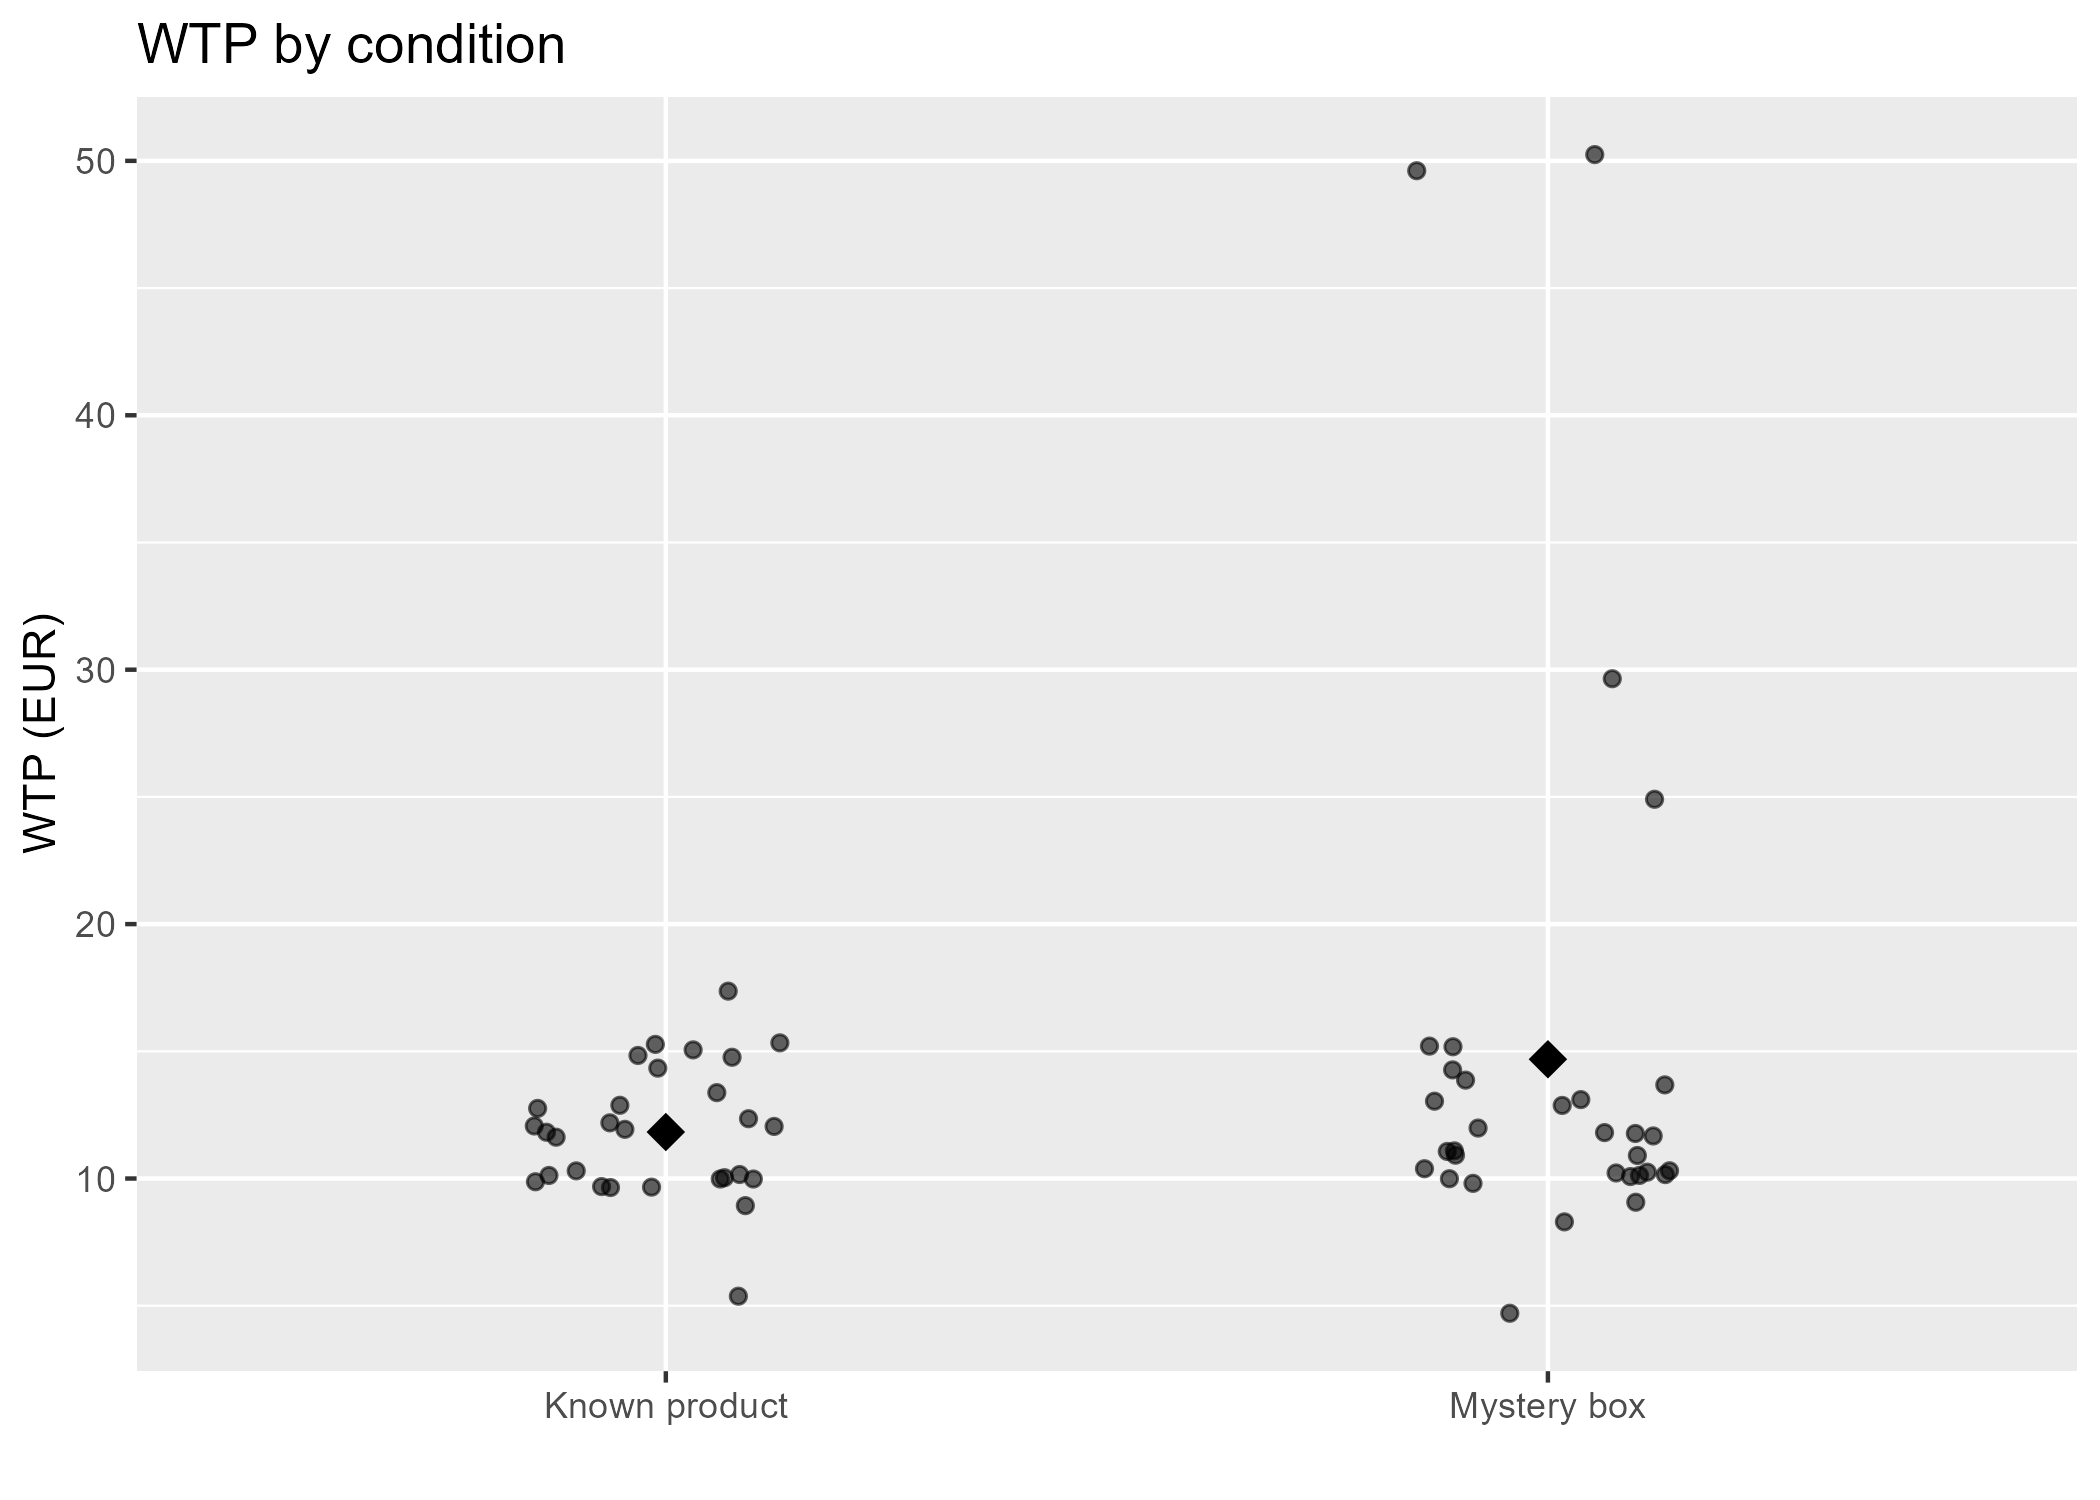
\includegraphics[width=0.9\textwidth]{wtp_points_means.png}
\caption{Willingness to pay by experimental condition}
\label{fig:wtp_condition}
\end{figure}

\section{Conclusion}

This project investigated the effect of product uncertainty on consumer valuation using a simple experiment comparing willingness to pay for a known chocolate product and a mystery chocolate box.

The experimental design allowed us to isolate the role of uncertainty while holding the general product category constant. Data were collected from a heterogeneous sample of 61 respondents, including students and adult participants who voluntarily completed the online survey.

\textbf{The descriptive analysis shows that willingness to pay for the mystery box is, on average, higher than for the known product.}

This difference is caused by a small group of respondents who report very high valuations. Importantly, \textbf{uncertainty does not increase valuations in the same way for all participants. Instead, it leads to greater variation and more polarized responses.} Some individuals stay close to the suggested price range, while others are willing to pay much higher amounts, even though they were informed that the expected value is between 10 and 15 euros.

This increase in variance is a central finding of the analysis and highlights a key behavioral mechanism: uncertainty appears to generate additional utility for certain consumers, likely through curiosity, anticipation, or optimistic beliefs about possible outcomes. At the same time, other consumers do not substantially revise their valuations, resulting in greater heterogeneity under the mystery condition. These results are consistent with behavioral theories emphasizing affective responses and probability weighting under uncertainty, rather than standard expected utility maximization.

The analysis also reveals interesting patterns across individual characteristics. Gender differences emerge in stated valuations, with \textbf{female respondents on average reporting slightly higher willingness to pay for the mystery box than male respondents}, although the sample size limits strong statistical conclusions. Prior experience with mystery products is associated with higher and more stable valuations, suggesting that familiarity may reduce ambiguity and shape expectations.\textbf{ Differences in self-reported seriousness and consumption habits across conditions further indicate that uncertainty may increase engagement with the task}, which can translate into higher stated valuations.

Overall, the findings suggest that mystery products can meaningfully affect consumer behavior by altering not only average willingness to pay but also the distribution of valuations. The results illustrate how \textbf{uncertainty can act as a source of utility rather than merely a source of risk}. At the same time, several limitations should be acknowledged. The use of a convenience sample, hypothetical willingness to pay, and an online survey environment may affect external validity. Future research could extend this analysis using incentivized laboratory experiments or field settings to better capture real purchasing behavior.

Despite these limitations, \textbf{the project provides clear evidence that uncertainty embedded in mystery boxes plays an important role in consumer decision-making.} The results contribute to the broader behavioral literature by highlighting the dual effect of uncertainty: increasing average valuation for some consumers while simultaneously amplifying disagreement across individuals.

\begin{thebibliography}{99}

\bibitem{KahnemanTversky1979}
Kahneman, D. and Tversky, A. (1979).
Prospect Theory: An Analysis of Decision under Risk.
\emph{Econometrica}, 47(2), 263--291.


\bibitem{Cordes2024}
Cordes, S. et al. (2024).
What Drives Demand for Loot Boxes? An Experimental Study.
\emph{Journal of Economic Behavior \& Organization}, forthcoming.

\bibitem{Zhang2022}
Zhang, Y. et al. (2022).
The Effect of Blind Box Product Uncertainty on Consumers' Purchase Intention.
\emph{Frontiers in Psychology}, 13, Article 123456.

\bibitem{Gong2024}
Gong, X. et al. (2024).
Unveiling the Enigma of Blind Box Impulse Buying: The Role of Curiosity.
\emph{Heliyon}, 10(3), e12345.

\end{thebibliography}


\end{document}